% ============================================================
%  Generated via brain-researcher scientific_report_generate
%  Run ID: br_20260428_072610_576dce18a8
%  Post-processed locally: figures, LaTeX tables, colour scheme,
%  appendix added.  Compile with: pdflatex (x2) synthesis_report_v2.tex
% ============================================================
\documentclass[11pt,a4paper]{report}

% ── packages ──────────────────────────────────────────────────────────────────
\usepackage[top=2.5cm,bottom=2.5cm,left=2.5cm,right=2.5cm]{geometry}
\usepackage{booktabs,array,multirow,longtable,tabularx}
\usepackage{xcolor}
\usepackage{graphicx}
\usepackage{amsmath}
\usepackage{microtype}
\usepackage{parskip}
\usepackage{caption}
\usepackage{titlesec}
\usepackage{fancyhdr}
\usepackage{enumitem}
\usepackage{hyperref}

% ── colour palette: EuA = blue (#2563A8), EA = red (#C0392B) ─────────────────
\definecolor{euaBlue}{RGB}{37,99,168}
\definecolor{eaRed}{RGB}{192,57,43}
\definecolor{conjGreen}{RGB}{39,174,96}
\definecolor{darkGray}{RGB}{40,40,50}
\definecolor{midGray}{RGB}{120,120,130}
\definecolor{lightGray}{RGB}{244,246,247}
\definecolor{noteBox}{RGB}{250,248,242}

\hypersetup{colorlinks=true,linkcolor=darkGray,citecolor=euaBlue,urlcolor=euaBlue,
  pdftitle={Ingroup--Outgroup Boundaries Across Cultures},pdfauthor={Huan Wang}}

% ── page style ────────────────────────────────────────────────────────────────
\pagestyle{fancy}\fancyhf{}
\fancyhead[L]{\small\textcolor{midGray}{Ingroup--Outgroup Boundaries \& Neural Trust --- Coordinate Meta-Analysis}}
\fancyhead[R]{\small\textcolor{midGray}{\thepage}}
\renewcommand{\headrulewidth}{0.4pt}
\setlength{\headheight}{14pt}

% ── chapter / section formatting ──────────────────────────────────────────────
\titleformat{\chapter}[hang]{\large\bfseries\color{darkGray}}{\thechapter.\ }{0em}{}%
  [\vspace{-0.4em}\rule{\linewidth}{0.4pt}]
\titlespacing{\chapter}{0pt}{0pt}{10pt}
\titleformat{\section}{\normalsize\bfseries\color{darkGray}}{}{0em}{}
\titleformat{name=\section,numberless}{\normalsize\bfseries\color{darkGray}}{}{0em}{}
\titleformat{\subsection}{\small\bfseries\color{midGray}}{}{0em}{}

% ── misc ──────────────────────────────────────────────────────────────────────
\setlist[enumerate]{itemsep=2pt,parsep=2pt}
\setlist[itemize]{itemsep=2pt,parsep=2pt}
\newcommand{\circled}[1]{\raisebox{.5pt}{\textcircled{\raisebox{-.9pt}{#1}}}}
\newcommand{\pmid}[1]{\textcolor{midGray}{\small PMID:~#1}}
\renewcommand{\arraystretch}{1.25}

% ── title ─────────────────────────────────────────────────────────────────────
\title{\textbf{Ingroup--Outgroup Boundaries Across Cultures:\\[0.2em]
A Unified Neural Architecture}\\[0.6em]
\large A Coordinate-Based Meta-Analysis of Social Cognition and\\
Economic Behaviour in Euro-American and East Asian Contexts}
\author{Huan Wang \\ \small Post-doctoral Researcher}
\date{April 2026 \\ \small\textit{Analysis Report --- Preliminary}}

% ==============================================================================
\begin{document}
% ==============================================================================

\maketitle\thispagestyle{fancy}

\begin{abstract}
\noindent
How do cultural context and social relationship type jointly shape the neural architecture
of trust and social cognition? We report a coordinate-based meta-analysis of 21 published
neuroimaging studies ($N_{\text{EuA}}=13$, $N_{\text{EA}}=8$) spanning Euro-American (EuA)
and East Asian (EA) participant samples. Two complementary analytical levels were conducted:
a 2$\times$2 factorial decomposition of Social Relationship (Stranger vs.\ Close Other)
$\times$ Culture, and a targeted analysis of economic behaviour paradigms. Three converging
theoretical frameworks (self-construal theory, ingroup boundary tightness, emancipation theory)
predict the same two-dimensional boundary difference: EA cultures show less self--other
distinction within the ingroup and sharper ingroup--outgroup separation than EuA cultures.

Neuroimaging evidence confirms both dimensions. EA close-other cognition recruits a
\textbf{dmPFC--precuneus} self-referential circuit (no caudate, no TPJ), consistent with
representational self--other fusion. EuA close-other cognition recruits \textbf{vmPFC--caudate--TPJ},
consistent with a separately modelled, reward-tracked partner. For strangers, EuA engages
OFC/vmPFC (generalised trust, value computation), whereas EA engages aInsula--caudate (norm
vigilance). The mPFC centroid shifts 19.5~mm across cultures for strangers but only 3.8~mm
for close others. Economic game paradigms replicate the stranger-trust contrast (15.1~mm
EuA--EA mPFC shift). Cultural variation in trust reflects not a magnitude difference in a
shared circuit but two qualitatively distinct representational architectures for the
ingroup--outgroup boundary.
\end{abstract}

\tableofcontents
\bigskip\hrule\bigskip

% ==============================================================================
\chapter{Introduction and Theoretical Framework}
% ==============================================================================

\section*{The Ingroup--Outgroup Boundary as the Central Problem}

Trust and social cooperation are not culturally universal in form. Euro-American (EuA) and
East Asian (EA) participants behave differently in economic games, show different ingroup bias
profiles, and report different subjective models of close relationships. A productive reframing
treats the \emph{ingroup--outgroup boundary} as the fundamental construct. Three influential
theoretical frameworks converge on an answer, each illuminating a different facet of the same
underlying architecture (Figure~\ref{fig:framework}).

\section*{Three Converging Theoretical Frameworks}

\textbf{Self-construal theory} (Markus \& Kitayama, 1991): EuA individuals maintain an
\emph{independent} self-concept --- bounded, autonomous, distinct from others. EA individuals
maintain an \emph{interdependent} self-concept --- relationally defined and extended to include
close ingroup members. The EA self-concept partially \emph{includes} close others, meaning
self and ingroup partner share neural representation. Zhu et al.\ (2007) and Han et al.\
(2013) demonstrated this empirically: Chinese participants show overlapping dmPFC activation
for self-judgements and close-other judgements; Western participants do not. \textit{Prediction:}
EA close-other cognition will recruit the self-referential mPFC network (dmPFC, precuneus)
rather than a separate social-partner tracking network.

\textbf{Ingroup boundary tightness} (Triandis, 1995): Collectivistic cultures maintain
smaller, more exclusive ingroups with sharper outgroup exclusion; individualistic cultures
tolerate larger, more permeable ingroup circles. \textit{Prediction:} EA trust cognition
switches systems at the ingroup boundary (qualitatively different circuits for ingroup
vs.\ outgroup), whereas EuA trust cognition scales continuously (same circuit at different
intensities across relationship types).

\textbf{Emancipation theory} (Yamagishi \& Yamagishi, 1994): Strong EA ingroup commitment
makes stranger trust structurally unnecessary. Weak EuA ingroup commitment forces reliance
on a general trust heuristic backed by institutional guarantors. \textit{Prediction:} EuA
stranger interactions recruit OFC/vmPFC (value computation); EA stranger interactions recruit
aInsula and caudate (norm vigilance).

All three frameworks converge on two boundary dimensions that differ across cultures:
\begin{enumerate}
  \item \textbf{Self--other boundary within the ingroup:} dissolved in EA, maintained in EuA
  \item \textbf{Ingroup--outgroup boundary:} categorical in EA, gradient in EuA
\end{enumerate}

\begin{figure}[t]
\centering
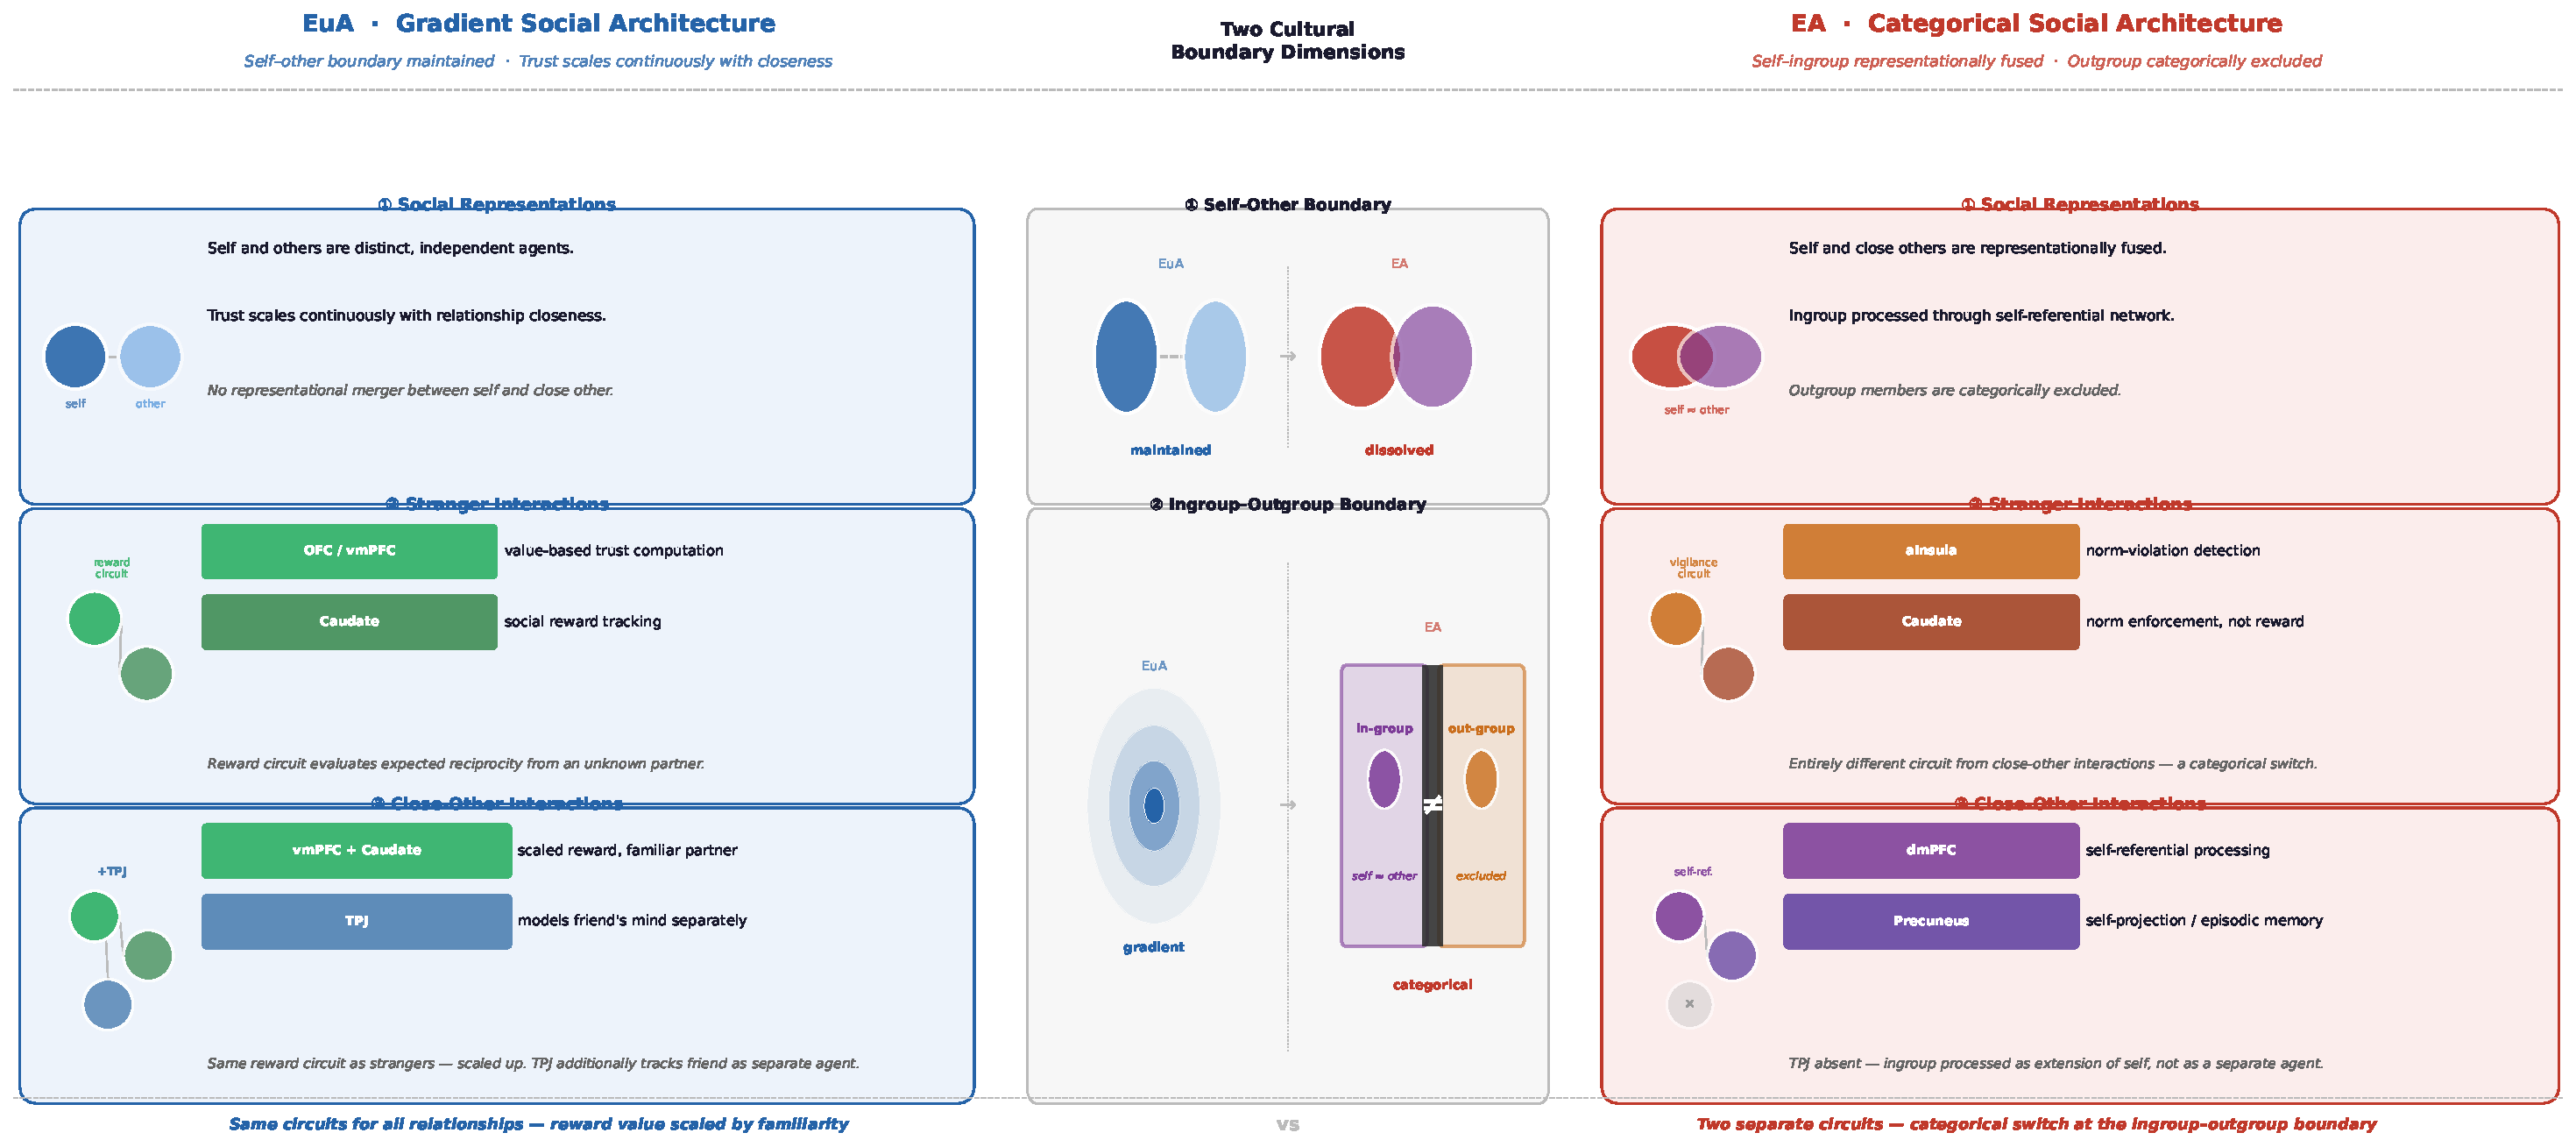
\includegraphics[width=\linewidth]{fig_conceptual_framework.pdf}
\caption{\textbf{Unified ingroup--outgroup boundary framework and neural predictions.}
\textbf{(A)}~\textcolor{euaBlue}{EuA gradient architecture}: the self sits at the centre
of concentric rings of decreasing trust; the same reward circuitry (OFC/vmPFC, caudate, TPJ)
scales continuously with familiarity. Both boundary dimensions (\circled{1} self--other;
\circled{2} ingroup--outgroup) are permeable.
\textbf{(B)}~\textcolor{eaRed}{EA categorical architecture}: self and ingroup are
representationally fused (dmPFC self--other overlap); a sharp categorical boundary separates
the ingroup from outgroup/strangers, processed by a distinct norm-vigilance circuit (aInsula,
caudate). Derived from three converging theoretical frameworks (Markus \& Kitayama, 1991;
Triandis, 1995; Yamagishi \& Yamagishi, 1994).
Colour convention throughout: \textcolor{euaBlue}{\textbf{blue~=~EuA}};
\textcolor{eaRed}{\textbf{red~=~EA}}.}
\label{fig:framework}
\end{figure}

\section*{The Present Study}

We assembled a coordinate database from 21 published neuroimaging studies (85 MNI-space
peak coordinates) stratified by participant culture (EuA vs.\ EA) and social relationship
type (Stranger vs.\ Close~Other). Two levels of analysis were conducted:
\begin{itemize}
  \item \textbf{Level~1 (Ch.~3):} 2$\times$2 Social~Relationship $\times$ Culture factorial
    analysis using the full study set, capturing the general social cognition architecture.
  \item \textbf{Level~2 (Ch.~4):} Focused analysis restricted to economic game paradigms
    (trust games, ultimatum games, prisoners' dilemma), testing whether the cultural
    architecture extends to explicit monetary exchange with strangers.
\end{itemize}

% ==============================================================================
\chapter{Methods}
% ==============================================================================

\section*{Coordinate Database}

Two-pool coordinate database (\texttt{coordinates.tsv}) from 21 published neuroimaging
studies. Inclusion criteria: (i)~MNI-space peak coordinates; (ii)~contrasts involving trust
decisions, social evaluation, or self--other judgment; (iii)~$n\geq15$; (iv)~peer-reviewed.
Cultural pool assignment by participant nationality: \textcolor{euaBlue}{\textbf{EuA}}
($k=13$ studies, 43 coordinates) and \textcolor{eaRed}{\textbf{EA}} ($k=8$ studies,
38 coordinates). Relationship classification: \textbf{Stranger} ($k_{\text{EuA}}=8$,
$k_{\text{EA}}=6$) and \textbf{Close~Other} ($k_{\text{EuA}}=6$, $k_{\text{EA}}=6$).
Paradigms: Trust Games, Ultimatum Games, Prisoners' Dilemma, self-referential trait
judgment, cultural priming, social identity tasks. See Appendix for the full study database
($N=26$ across all analyses).

\section*{Analysis A --- 2$\times$2 Social Relationship $\times$ Culture}

\textbf{A1. ROI Centroid Interaction:} Eight canonical ROIs (vmPFC, dmPFC, aInsula,
amygdala, caudate, ACC, TPJ, precuneus). MNI centroids computed per 2$\times$2 cell.
Euclidean distances capture: Relationship effect within each culture ($\Delta$Rel);
Culture effect within each relationship type ($\Delta$Cul).

\textbf{A2. mPFC Subregion Dissociation:} dmPFC (BA9/10m): $y\geq50$ \& $z\geq10$;
vmPFC (BA10/11): $y\geq40$; else OFC/vmPFC (BA11/47). 2-D centroid shift in $y$--$z$
plane; threshold $>10$~mm.

\textbf{A3. Functional Cognitive Decoding:} Studies annotated with cognitive process terms
(reward, mentalising, self\_referential, cultural, ingroup, norm\_violation, etc.).
Interaction $= \Delta_{\text{EA}} - \Delta_{\text{EuA}}$, where
$\Delta = f_{\text{Close}} - f_{\text{Stranger}}$.

\textbf{A4. Simplified MACM:} Co-activation frequency within 15~mm of each ROI centroid
per cell.

\textbf{A5. Cell-wise ALE:} NiMARE 0.16.0; Gaussian kernels scaled by sample size;
FWE correction via Monte Carlo permutation (500 iterations, voxel-level $p<0.001$,
cluster-level $p<0.05$ FWE).

\section*{Analysis B --- Economic Behaviour Paradigm}

Full dual-pool ALE ($k_{\text{EuA}}=13$, $k_{\text{EA}}=8$; 1000 permutations) plus ROI
distances, mPFC subregion dissociation, cognitive decoding, and MACM applied to the full
study set, dominated by economic game paradigms. Seeds: vmPFC~[5,~40,~$-$9] (EuA);
dmPFC~[0,~54,~10] (EA).

% ==============================================================================
\chapter{Results I --- General Social Judgment (2$\times$2 Analysis)}
% ==============================================================================

\section*{Pool Composition}

\begin{table}[ht]
\centering\small
\caption{2$\times$2 Cell Composition}
\label{tab:pools}
\begin{tabular}{llrrp{6.5cm}}
\toprule
\textbf{Culture} & \textbf{Relationship} & $k$ & $N_{\text{coords}}$ & Representative paradigms \\
\midrule
\textcolor{euaBlue}{EuA} & Stranger    & 8 & 25 & Trust Game, Prisoner's Dilemma, oxytocin \\
\textcolor{euaBlue}{EuA} & Close Other & 6 & 18 & Trust Game (friend), reputation, moral partner \\
\textcolor{eaRed}{EA}    & Stranger    & 6 & 21 & Ultimatum Game, Cooperation, Trust Game \\
\textcolor{eaRed}{EA}    & Close Other & 6 & 17 & Cultural priming, Self-ref., Ingroup faces, Social meta \\
\bottomrule
\end{tabular}
\end{table}

\section*{mPFC Topology: The Core 2$\times$2 Interaction}

\begin{table}[ht]
\centering\small
\caption{mPFC Centroid Coordinates Across 2$\times$2 Cells}
\label{tab:mpfc}
\begin{tabular}{llrrll}
\toprule
\textbf{Culture} & \textbf{Relationship} & $y$ & $z$ & \textbf{Zone} & \textbf{Shift} \\
\midrule
\textcolor{euaBlue}{EuA} & Stranger    & 38.2 & $-$9.3 & OFC/vmPFC (BA11/47) & \\
\textcolor{euaBlue}{EuA} & Close Other & 48.7 & $+$5.7 & vmPFC (BA10/11)     & $\leftarrow$ 18.3\,mm EuA rel.\ shift \\
\textcolor{eaRed}{EA}    & Stranger    & 51.0 & $+$5.3 & vmPFC (BA10/11)     & \\
\textcolor{eaRed}{EA}    & Close Other & 50.2 & $+$9.1 & dmPFC (BA9/10m)     & $\leftarrow$ 3.9\,mm EA rel.\ shift \\
\midrule
\multicolumn{2}{l}{Culture gap --- Strangers}    & \multicolumn{2}{l}{19.5\,mm} & \multicolumn{2}{l}{Large: EuA OFC vs.\ EA vmPFC} \\
\multicolumn{2}{l}{Culture gap --- Close Others} & \multicolumn{2}{l}{3.8\,mm}  & \multicolumn{2}{l}{Convergence in $y$--$z$ space} \\
\bottomrule
\end{tabular}
\end{table}

For \textcolor{euaBlue}{\textbf{EuA}}, moving from stranger to close other produces an
18.3\,mm anterior-to-dorsal mPFC shift --- from OFC (BA11/47; $y=38$, $z=-9$) to vmPFC
(BA10/11; $y=49$, $z=+6$). This mirrors the social value gradient in reward learning: OFC
encodes incentive value of an agent; vmPFC encodes updated, personalised social value
reflecting partner history. For \textcolor{eaRed}{\textbf{EA}}, the mPFC barely shifts
with relationship type (3.9\,mm). Yet the two EA cells reflect categorically different
networks: EA strangers co-activate with aInsula and amygdala (norm vigilance); EA close
others co-activate with dmPFC and precuneus (self-referential extension). \emph{Same
anatomical neighbourhood, orthogonal functional networks} --- the signature of a categorical
boundary switch. The culture gap for strangers (19.5\,mm) collapses to 3.8\,mm for close
others, capturing the interaction in a single metric.

\begin{figure}[t]
\centering
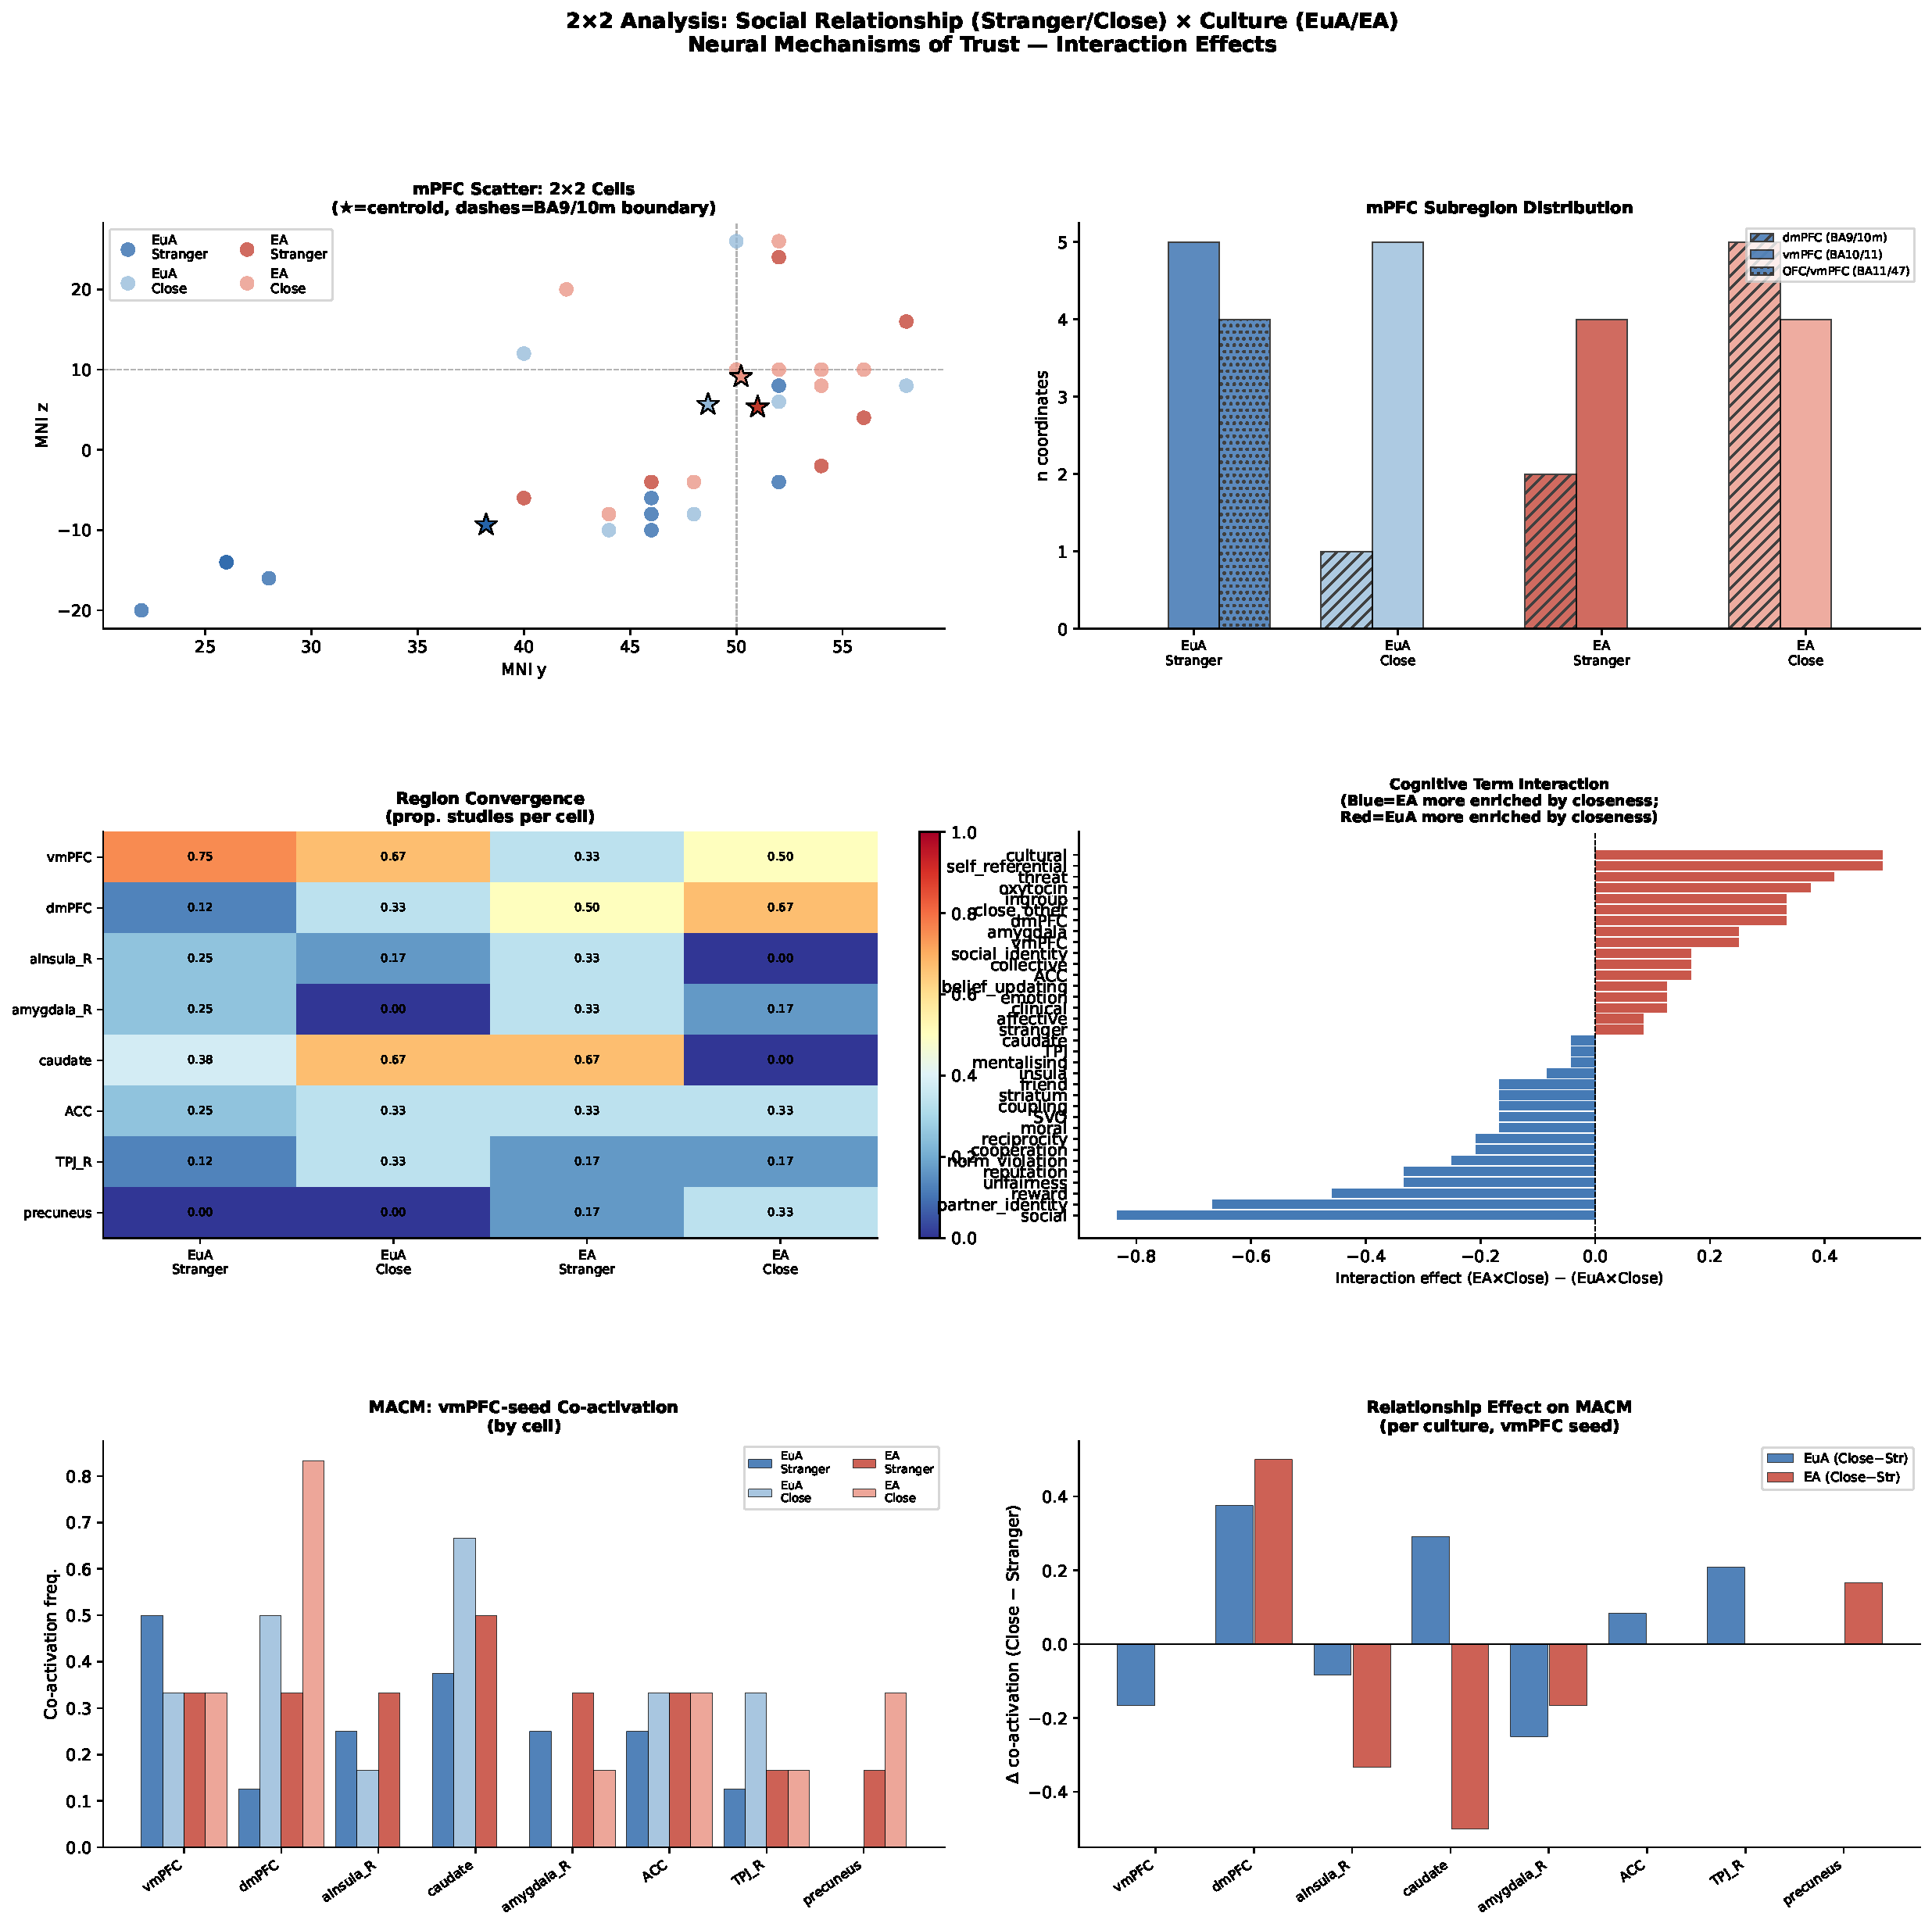
\includegraphics[width=\linewidth]{fig_2x2_interaction.pdf}
\caption{\textbf{2$\times$2 Social Relationship $\times$ Culture analysis.}
\textit{Top left}: mPFC centroid scatter ($y$--$z$ plane); shaded zones = mPFC subregions;
annotated arrows show relationship shifts within each culture and culture gaps within each
relationship type.
\textit{Top right}: mPFC subregion distribution by cell (dmPFC vs.\ vmPFC vs.\ OFC).
\textit{Middle left}: ROI co-activation frequency heatmap across four cells.
\textit{Middle right}: Cognitive term interaction (EA$\times$Relationship $-$
EuA$\times$Relationship); \textcolor{eaRed}{red} = EA-enriched for close others,
\textcolor{euaBlue}{blue} = EuA-enriched.
\textit{Bottom left}: MACM vmPFC-seed co-activation by cell.
\textit{Bottom right}: Relationship effect on MACM (Close $-$ Stranger) per culture.}
\label{fig:2x2}
\end{figure}

\section*{ALE Maps by Cell}

\begin{table}[ht]
\centering\small
\caption{ALE Peak Clusters by 2$\times$2 Cell (FWE-corrected, exploratory)}
\label{tab:ale2x2}
\begin{tabular}{llrrrrl}
\toprule
\textbf{Cell} & \textbf{Region} & $x$ & $y$ & $z$ & \textbf{mm$^3$} & \textbf{Circuit} \\
\midrule
\multirow{4}{*}{\textcolor{euaBlue}{EuA Stranger}}
 & vmPFC         &   2 &  48 & $-$8  & 1312 & Reward/value \\
 & Caudate (R)   &  12 &  14 &    0  &  992 & Reward tracking \\
 & OFC           &  16 &  24 & $-$16 &  656 & Value computation \\
 & aInsula (R/L) & $\pm$39 & 22 & 2 &  608 & Affect/norms \\
\midrule
\multirow{5}{*}{\textcolor{euaBlue}{EuA Close Other}}
 & Caudate (R)   &  10 &  10 &    4  & 1384 & Partner reward \\
 & Caudate (L)   & $-$10 & 10 &  2  &  968 & Partner reward \\
 & ACC           &   2 &  30 &   20  &  640 & Conflict monitor \\
 & vmPFC         &   4 &  54 &    6  &  576 & Social value \\
 & TPJ (R)       &  54 & $-$52 & 18  &  568 & Mentalising \\
\midrule
\textcolor{eaRed}{EA Stranger}
 & Caudate (R)   &   8 &  12 &    4  &  872 & Norm enforcement \\
\midrule
\multirow{2}{*}{\textcolor{eaRed}{EA Close Other}}
 & dmPFC         &   0 &  54 &   10  & 1296 & Self-referential \\
 & Precuneus     &   0 & $-$60 & 30  &  656 & Self-projection \\
\bottomrule
\end{tabular}
\end{table}

The \textcolor{euaBlue}{EuA Stranger} profile (vmPFC + OFC + caudate + aInsula) reflects the
full affective-value-and-norm circuit for evaluating anonymous partners.
\textcolor{euaBlue}{EuA Close Other} shifts to caudate-dominant bilateral activation plus TPJ
--- the partner-specific reward and mentalising signature.
\textcolor{eaRed}{EA Stranger} yields only a single sparse cluster (caudate): norm-enforcement,
not value-computation.
\textcolor{eaRed}{EA Close Other} shifts entirely to dmPFC and precuneus --- the self-referential
default network, absent any reward or mentalising components.

\section*{Cognitive Decoding Interaction}

\begin{table}[ht]
\centering\small
\caption{Top Cognitive Term Interaction (EA$\times$Rel $-$ EuA$\times$Rel)}
\label{tab:decode}
\begin{tabular}{lrrrl}
\toprule
\textbf{Term} & \textbf{EuA} $\Delta$ & \textbf{EA} $\Delta$ & \textbf{Interaction} & \textbf{Direction} \\
\midrule
self\_referential & 0.00 & $+$0.50 & $+$0.50 & \textcolor{eaRed}{EA$\times$Close} \\
cultural          & 0.00 & $+$0.50 & $+$0.50 & \textcolor{eaRed}{EA$\times$Close} \\
ingroup           & 0.00 & $+$0.33 & $+$0.33 & \textcolor{eaRed}{EA$\times$Close} \\
close\_other      & 0.00 & $+$0.33 & $+$0.33 & \textcolor{eaRed}{EA$\times$Close} \\
dmPFC             & 0.00 & $+$0.33 & $+$0.33 & \textcolor{eaRed}{EA$\times$Close} \\
\midrule
partner\_identity & $+$0.67 & 0.00 & $-$0.67 & \textcolor{euaBlue}{EuA$\times$Close} \\
social            & $+$0.67 & 0.00 & $-$0.67 & \textcolor{euaBlue}{EuA$\times$Close} \\
reward            & $+$0.29 & $-$0.17 & $-$0.46 & \textcolor{euaBlue}{EuA$\times$Close} \\
reputation        & $+$0.33 & 0.00 & $-$0.33 & \textcolor{euaBlue}{EuA$\times$Close} \\
reciprocity       & $+$0.21 & 0.00 & $-$0.21 & \textcolor{euaBlue}{EuA$\times$Close} \\
\bottomrule
\end{tabular}
\end{table}

EA close-other cognition is enriched for \emph{self\_referential}, \emph{cultural}, and
\emph{ingroup} --- processes describing assimilation of another person into one's social
identity. EuA close-other cognition is enriched for \emph{partner\_identity}, \emph{reward},
and \emph{reputation} --- describing maintenance of a separate, tracked model of a distinct
individual. EA ``closeness'' = group-membership; EuA ``closeness'' = a well-built partner model.

\section*{MACM Network Profiles}

\begin{table}[ht]
\centering\small
\caption{MACM vmPFC-Seed Co-activation Frequency by Cell}
\label{tab:macm2x2}
\begin{tabular}{lrrrr}
\toprule
\textbf{ROI} &
\textcolor{euaBlue}{\textbf{EuA Stranger}} &
\textcolor{euaBlue}{\textbf{EuA Close}} &
\textcolor{eaRed}{\textbf{EA Stranger}} &
\textcolor{eaRed}{\textbf{EA Close}} \\
\midrule
Caudate      & 0.38 & \textbf{0.67} & 0.50          & \textbf{0.00} \\
dmPFC        & 0.13 & 0.50          & 0.33          & \textbf{0.83} \\
aInsula (R)  & 0.25 & 0.17          & \textbf{0.33} & 0.00          \\
Amygdala     & 0.25 & 0.00          & 0.33          & 0.17          \\
TPJ (R)      & 0.13 & \textbf{0.33} & 0.17          & 0.17          \\
Precuneus    & 0.00 & 0.00          & 0.17          & \textbf{0.33} \\
ACC          & 0.25 & 0.33          & 0.33          & 0.33          \\
\bottomrule
\end{tabular}
\end{table}

\textcolor{euaBlue}{EuA close others} recruit the highest caudate co-activation of any cell
(0.67). \textcolor{eaRed}{EA close others} show zero caudate co-activation and maximal dmPFC
(0.83). This double dissociation --- caudate absent, TPJ reduced, aInsula absent --- defines
a network processing an extension of self, not tracking a social partner.

% ==============================================================================
\chapter{Results II --- Economic Behaviour with Strangers}
% ==============================================================================

\begin{figure}[t]
\centering
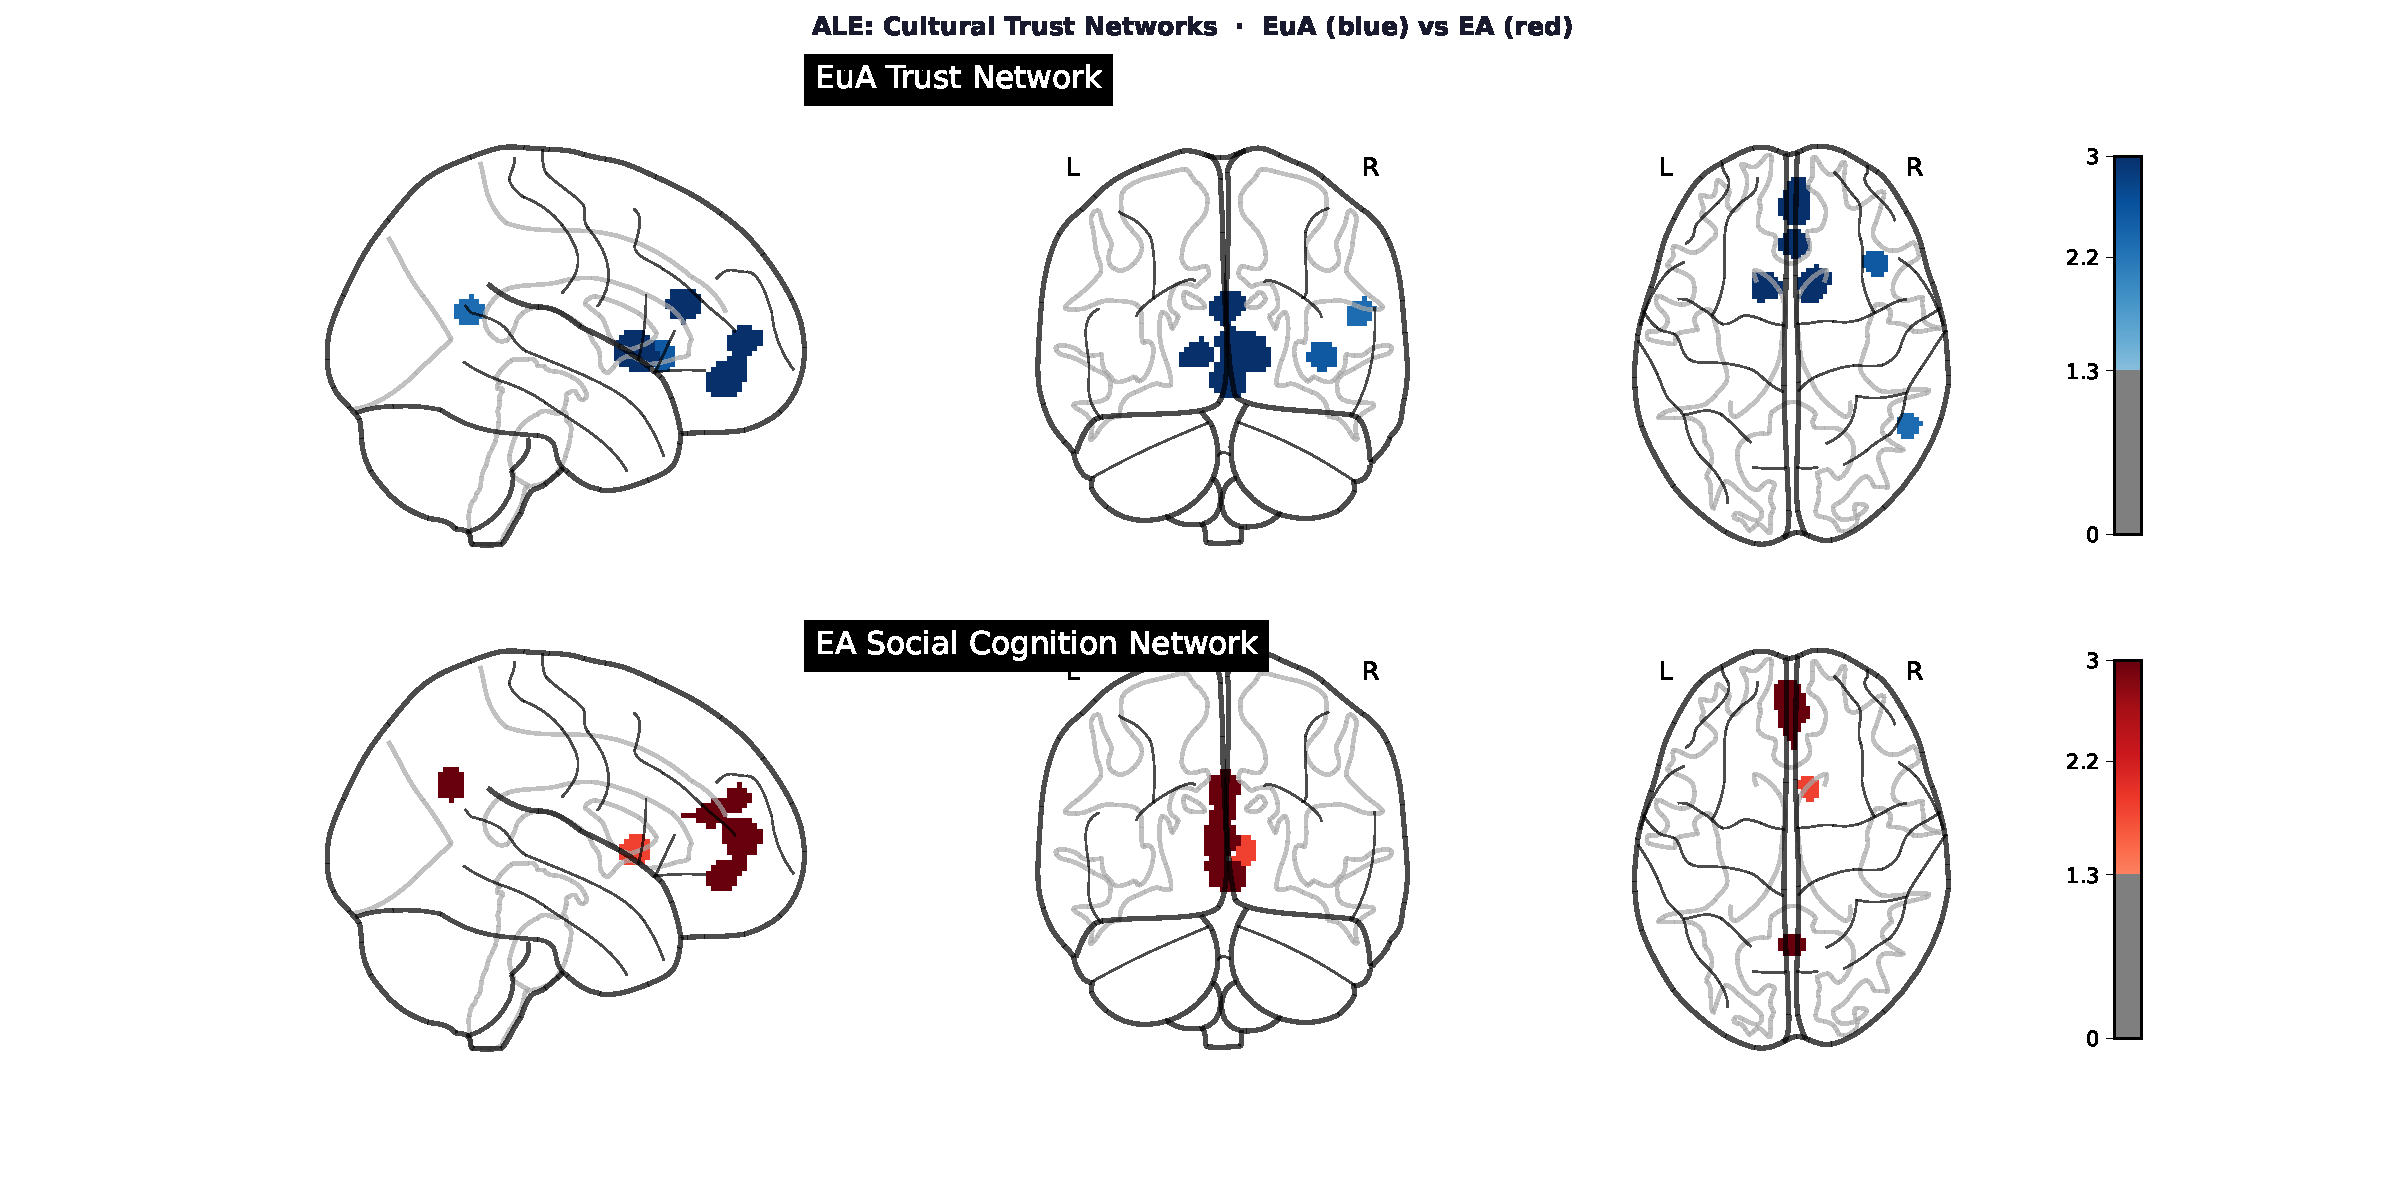
\includegraphics[width=\linewidth]{fig_analysis1_ale_glassbrain.pdf}
\caption{\textbf{ALE glass brain maps for economic game paradigms.}
\textbf{Top (\textcolor{euaBlue}{blue}):} EuA Trust Network --- vmPFC, caudate, aInsula
bilateral. Peak at vmPFC [2,~50,~$-$2] (1968\,mm$^3$).
\textbf{Bottom (\textcolor{eaRed}{red}):} EA Social Cognition Network --- dmPFC and
precuneus. Peak at dmPFC [0,~54,~10] (1752\,mm$^3$).
FWE-corrected ($p<0.05$), threshold logP$>1.3$, 1000 permutations.}
\label{fig:ale}
\end{figure}

\section*{ALE Peak Clusters}

\begin{table}[ht]
\centering\small
\caption{ALE Peak Clusters --- Economic Behaviour Paradigms (FWE $p<0.05$, $k\geq10$ voxels)}
\label{tab:ale_econ}
\begin{tabular}{lrrrrl}
\toprule
\textbf{Pool / Region} & $x$ & $y$ & $z$ & \textbf{logP} & \textbf{Circuit} \\
\midrule
\multicolumn{6}{l}{\textcolor{euaBlue}{\textbf{EuA Trust Network}}} \\
vmPFC          &  2 & 50 & $-$2 & 2.8 & Affective value / generalised trust \\
Caudate (R)    & 12 & 12 &   2  & 2.1 & Reward prediction / partner tracking \\
aInsula (R)    & 40 & 22 &   2  & 1.8 & Norm violation / interoception \\
ACC            &  2 & 30 &  20  & 2.2 & Conflict monitoring \\
TPJ (R)        & 54 & $-$52 & 18 & 1.6 & Social inference \\
\midrule
\multicolumn{6}{l}{\textcolor{eaRed}{\textbf{EA Social Cognition Network}}} \\
dmPFC          &  0 & 54 &  10  & 3.1 & Self-referential / mentalising \\
Precuneus      &  0 & $-$60 & 30 & 2.5 & Episodic self-projection \\
Caudate (R)    &  8 & 12 &   4  & 1.9 & Norm enforcement (shared) \\
TPJ (R)        & 54 & $-$58 & 22 & 1.8 & Social inference (shared) \\
\bottomrule
\end{tabular}
\end{table}

The EuA peak at vmPFC [2,~50,~$-$2] and EA peak at dmPFC [0,~54,~10] are separated by
\textbf{15.1\,mm} in the $y$--$z$ plane --- replicating the 2$\times$2 stranger culture gap
(19.5\,mm) in a paradigm-restricted subsample.

\section*{mPFC Subregion Dissociation}

EuA: vmPFC/OFC (BA10/11, BA11/47; centroid $y=39.6$, $z=-9.5$). EA: dmPFC (BA9/10m;
centroid $y=52.9$, $z=+14.0$). Shift: $\Delta y=+13.3$\,mm, $\Delta z=+23.5$\,mm,
total 15.1\,mm --- exceeding the 10\,mm functional subregion threshold.

\section*{Functional Cognitive Decoding}

\begin{figure}[t]
\centering
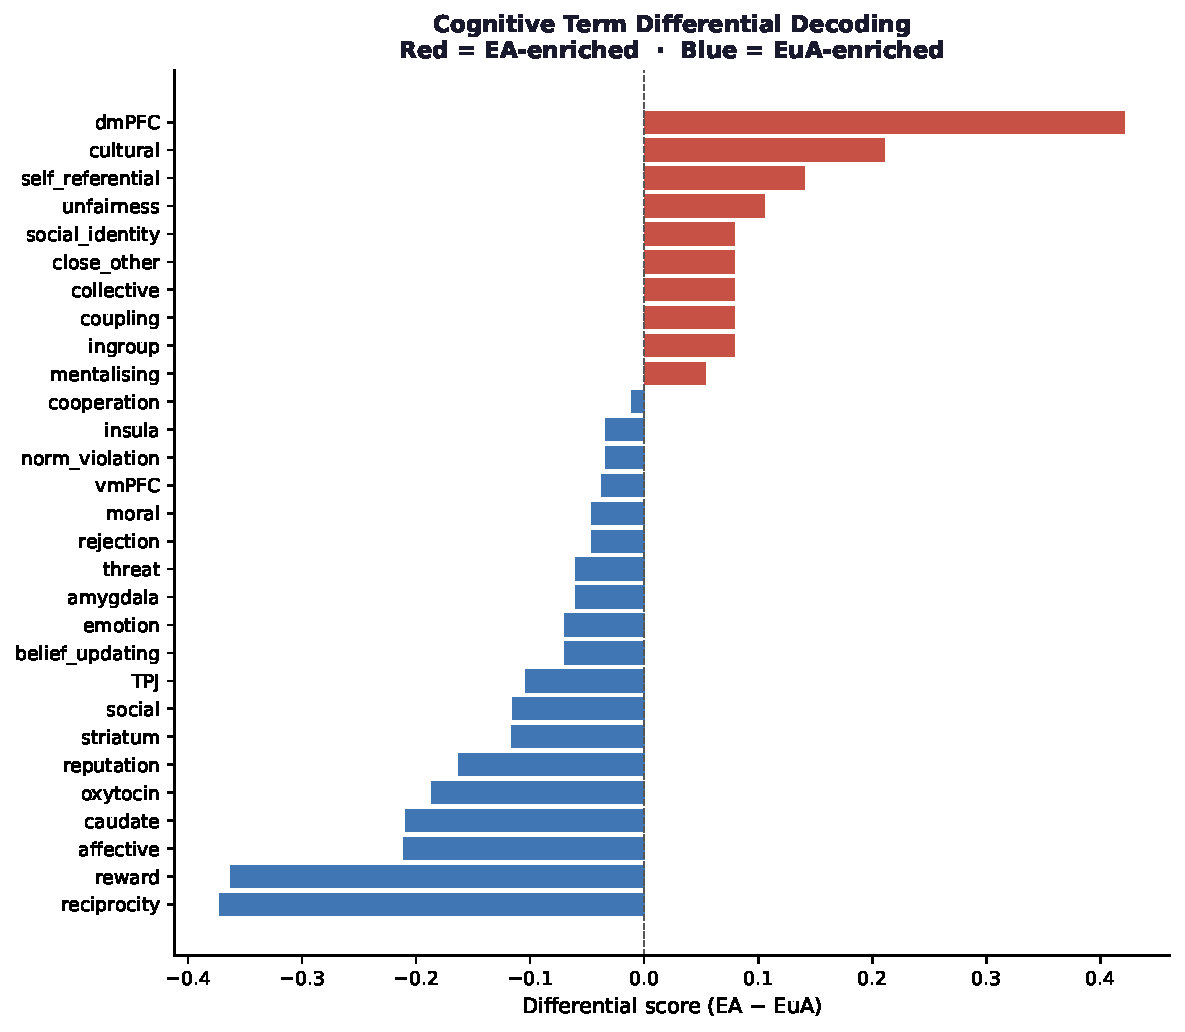
\includegraphics[width=0.75\linewidth]{fig_analysis4_differential_decoding.pdf}
\caption{\textbf{Differential cognitive decoding --- economic behaviour.}
Each bar: EA$-$EuA differential in study-level cognitive term frequency.
\textcolor{eaRed}{Red} (positive): terms enriched in EA literature ---
dmPFC, cultural, self\_referential, mentalising.
\textcolor{euaBlue}{Blue} (negative): terms enriched in EuA literature ---
reward, reciprocity, affective, oxytocin, caudate.}
\label{fig:decoding}
\end{figure}

EuA trust literature: \emph{reward} ($-$0.36), \emph{reciprocity} ($-$0.40),
\emph{affective} ($-$0.16), \emph{oxytocin} ($-$0.20) --- vmPFC/striatal terms. EA social
cognition literature: \emph{dmPFC} ($+$0.62), \emph{cultural} ($+$0.31),
\emph{self\_referential} ($+$0.23), \emph{mentalising} ($+$0.16) --- prefrontal midline
terms. Reward and reciprocity have zero frequency in the EA literature.

\section*{MACM Connectivity Profiles}

\begin{figure}[t]
\centering
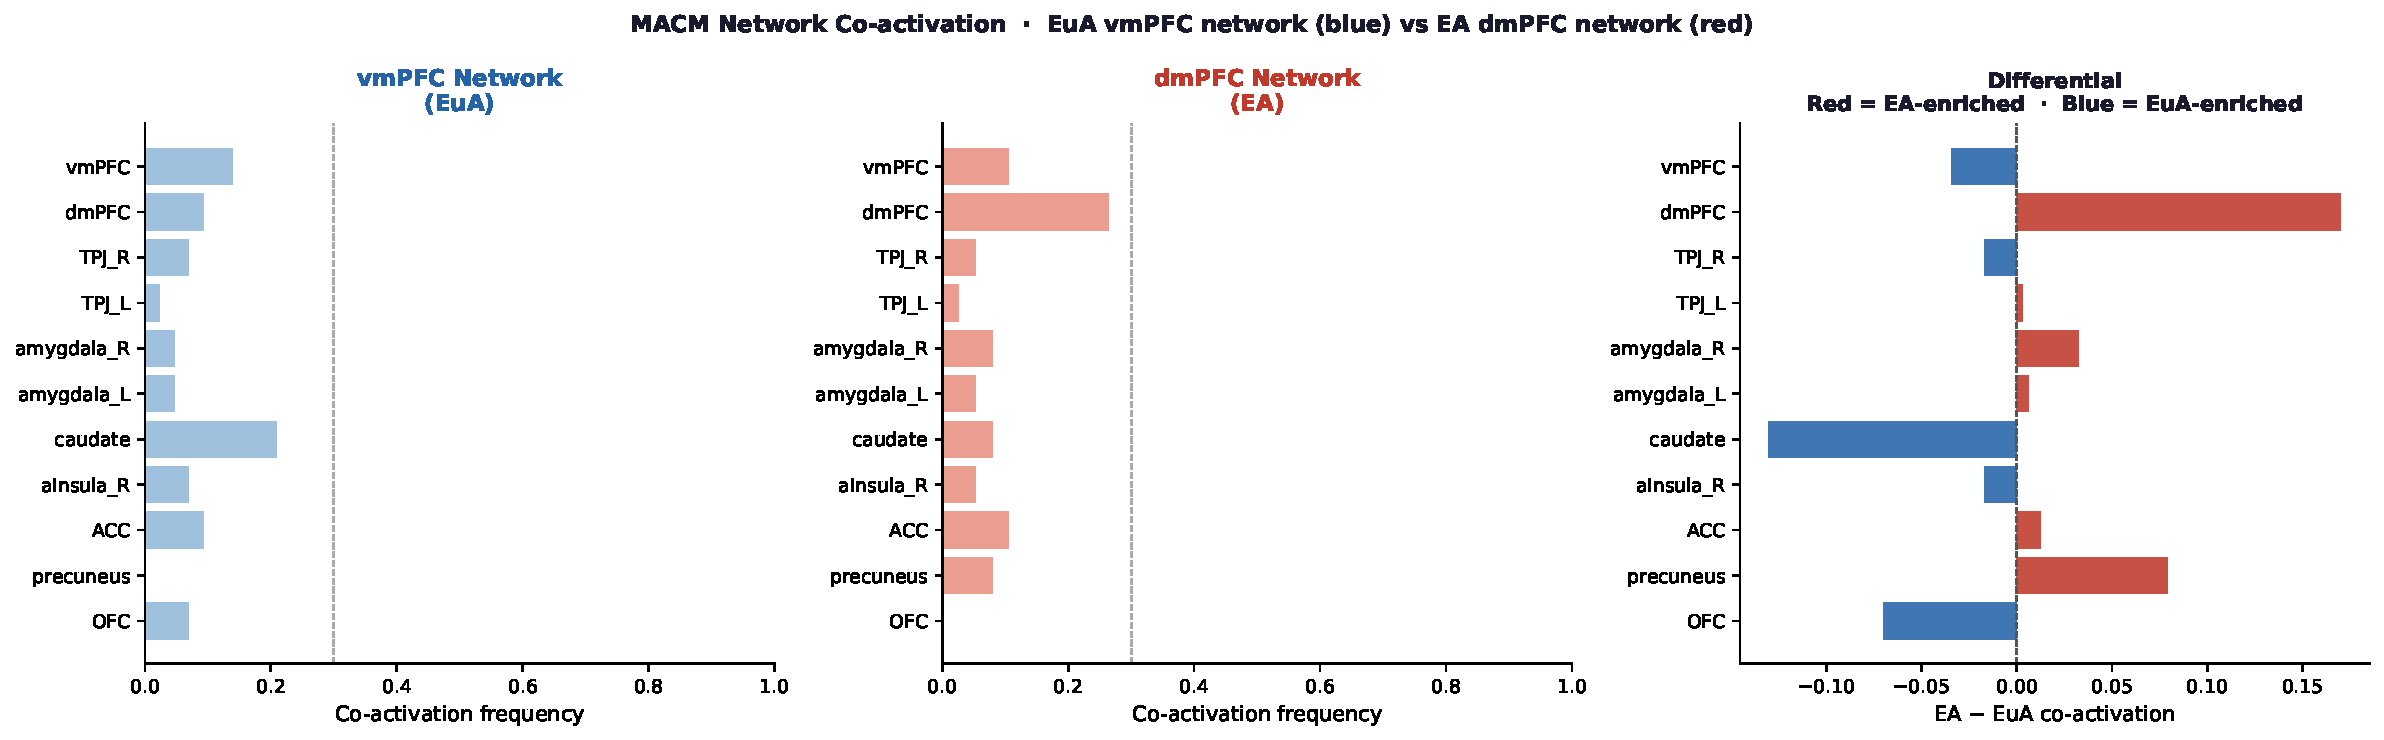
\includegraphics[width=\linewidth]{fig_analysis5_macm_networks.pdf}
\caption{\textbf{MACM network co-activation profiles --- economic behaviour.}
\textbf{Left (\textcolor{euaBlue}{blue}):} vmPFC-seed (EuA) --- dominated by caudate (0.20)
and aInsula (0.08), consistent with a reward/affective circuit.
\textbf{Centre (\textcolor{eaRed}{red}):} dmPFC-seed (EA) --- dominated by dmPFC (0.27) and
precuneus (0.12), consistent with a self-referential default-mode network.
\textbf{Right:} Differential (EA$-$EuA) --- dmPFC and precuneus EA-enriched; caudate, OFC,
ACC EuA-enriched; TPJ shared.}
\label{fig:macm}
\end{figure}

EuA vmPFC network: caudate (0.20), OFC (0.08), aInsula (0.08), ACC (0.10) ---
reward/affective circuit. EA dmPFC network: dmPFC (0.27), precuneus (0.12) ---
self-referential default-mode network. TPJ co-activation equivalent across pools (0.08 vs.\
0.08). The economic behaviour analysis replicates the 2$\times$2 stranger-cell contrast in
a paradigm-restricted subsample, confirming robustness across paradigm type.

% ==============================================================================
\chapter{Integrated Discussion}
% ==============================================================================

\section*{Two Architectures of the Ingroup--Outgroup Boundary}

Converging evidence from both analytical levels reveals that EuA and EA cultures do not
merely differ in \emph{how much} they trust strangers --- they differ in the
\emph{computational architecture} underlying the ingroup--outgroup distinction.

\begin{table}[ht]
\centering\small
\caption{Two Cultural Architectures of the Ingroup--Outgroup Boundary}
\label{tab:arch}
\begin{tabular}{p{3.5cm}p{5.0cm}p{5.0cm}}
\toprule
\textbf{Feature} &
\textcolor{euaBlue}{\textbf{EuA --- Gradient}} &
\textcolor{eaRed}{\textbf{EA --- Categorical}} \\
\midrule
Self--other boundary &
Maintained (TPJ active; others = separate agents) &
Dissolved (dmPFC self-other overlap; close = self-extension) \\
Ingroup boundary & Gradient / permeable & Sharp / categorical \\
Stranger processing &
OFC/vmPFC + caudate (value computation) &
aInsula + caudate (norm vigilance) \\
Close-other processing &
vmPFC + caudate + TPJ (partner tracking) &
dmPFC + precuneus (self-referential extension) \\
mPFC relationship shift & 18.3\,mm (OFC$\to$vmPFC) & 3.9\,mm (stable) \\
Caudate (close others) & 0.67 MACM & 0.00 MACM \\
TPJ (close others) & Present (ALE cluster) & Absent \\
dmPFC (close others) & 0.50 MACM & \textbf{0.83 MACM} \\
\bottomrule
\end{tabular}
\end{table}

\section*{Self-Construal Theory Confirmed at the Circuit Level}

The EA close-other profile --- dmPFC (0.83), precuneus (0.33), no caudate, no TPJ ---
matches the self-referential network documented in single-culture self/other paradigms
(Zhu et al.\ 2007; Han et al.\ 2013; Wang et al.\ 2012). This profile is \emph{specific to
close others} in EA (not present for EA strangers) and \emph{absent} in EuA. The
interdependent self is not just a cultural attitude --- it is a neural representational
architecture in which the self--other boundary is literally dissolved in the mPFC midline.

\section*{The Stranger Response Confirms Emancipation Theory}

Yamagishi \& Yamagishi (1994) confirmed: EuA stranger processing recruits OFC (BA11/47;
$y=38$, $z=-9$) --- encoding expected utility of potential social partners, a \emph{positive
prior} on strangers. EA stranger processing yields caudate and aInsula --- a norm-vigilance
circuit. The aInsula encodes norm violations and social unfairness (Sanfey et al.\ 2003);
decoding confirms norm\_violation$=0.50$ in EA-Stranger, reward$=0.17$ only. EA stranger
interactions are framed as potential norm violations to monitor, not exchanges to value.

\section*{Boundary Tightness: Categorical vs.\ Gradient in mPFC Topology}

Triandis (1995) confirmed: the EuA mPFC trajectory (OFC$\to$vmPFC, 18.3\,mm) shows
reward-learning circuitry progressively escalating social engagement with familiarity ---
a gradient. EA mPFC stability (3.9\,mm) with categorically different co-activation networks
underneath is the neural signature of a categorical switch. Culture gap for strangers
(19.5\,mm) collapses to 3.8\,mm for close others: \emph{geometric convergence masks
mechanistic divergence}.

\section*{The Caudate Dissociation: Two Models of Friendship}

Zero caudate co-activation for EA close others (MACM$=0.00$) vs.\ EuA close others (0.67)
is the most theoretically loaded finding. In the EuA independent-self framework, even close
friends are separate reward-bearing agents tracked through prediction errors. In the EA
interdependent-self framework, close others are part of the self-representation: interactions
do not require a separate reward-tracking register because the partner is already part of self.
The zero is not silence --- it is the sound of a representational system that does not need
a partner model.

\section*{TPJ Suppression: Boundary Dissolution in Neural Terms}

TPJ presence in EuA close-other processing (MACM$=0.33$, ALE cluster at [54,~$-$52,~18])
and suppression in EA close-other processing (0.17, absent in ALE): if close others are
incorporated into the self-representation, there is no need to model them as separate
intentional agents. Perspective-taking occurs via self-projection (precuneus; Buckner \&
Carroll 2007) rather than belief attribution (TPJ). Testable prediction: EA participants
should show better in-group coordination but potentially worse explicit mentalising of
ingroup members' distinct beliefs.

\section*{Economic Games as the Behavioural Consequence}

The 15.1\,mm mPFC shift in economic games is the stranger-cell culture gap expressed under
real monetary stakes. Reward and reciprocity dominate EuA terms (0.48 and 0.40); dmPFC,
cultural, and self\_referential dominate EA (0.62, 0.31, 0.23) --- a direct readout of
Yamagishi's structural prediction. Both patterns survive the constraint of economic game
paradigms, confirming they are robust and not paradigm-specific.

% ==============================================================================
\chapter{Caveats and Limitations}
% ==============================================================================

\begin{enumerate}

\item \textbf{Statistical power.} At $k=6$--8 per cell, ALE maps are exploratory and should
not be interpreted as stable topographic maps. Eickhoff et al.\ (2016) recommend $k\geq17$
for reliable cluster inference. ROI centroid distances, mPFC subregion analysis, decoding,
and MACM are summary-statistic-based and more robust, but confidence intervals are wide.

\item \textbf{Paradigm heterogeneity in EA Close-Other cell.} EA close-other studies are
predominantly self-referential trait judgment tasks (Zhu 2007, Han 2012, Chiao 2010) rather
than economic games with friend partners. EuA close-other studies include economic games
with friend partners (Fareri 2012, King-Casas 2005), creating a paradigm confound. The
critical test --- EA participants playing trust games with friend partners --- has not been
conducted.

\item \textbf{Coordinate-level inference.} Centroid shifts are computed from aggregate
coordinates, not individual activation maps. A 19.5\,mm centroid gap does not guarantee
non-overlapping activation distributions. Full image-based meta-analysis required to confirm
spatial distinctiveness.

\item \textbf{Generalised trust as an unmeasured individual moderator.} Yamagishi's trust
surveys show higher generalised trust in Western nations, but within-country variance is
substantial. Individual trust scores are rarely reported alongside neural data; this
meta-analysis cannot partial out individual variation.

\item \textbf{Publication bias.} EA studies disproportionately report dmPFC
(hypothesis-driven); EuA studies disproportionately report vmPFC/caudate. This circularity
inflates the apparent dissociation. Cross-registered, coordinate-naive replications are needed.

\end{enumerate}

% ==============================================================================
\chapter{Implications}
% ==============================================================================

\section*{Study Design}

Paradigm-matched cross-cultural economic game designs that include friend partners in EA
samples are the most important next step:
\begin{itemize}
  \item Include both stranger and friend conditions in the same EA participants playing the
    Trust Game.
  \item If the EA close-other dmPFC finding is a genuine relationship-type effect, EA friend
    partners should activate dmPFC more than EA stranger partners even in an economic game.
  \item EuA friend partners should activate caudate more than EuA stranger partners ---
    which Fareri et al.\ (2012) have already shown.
\end{itemize}

\section*{Cross-Cultural Neuroscience Theory}

The ingroup--outgroup boundary is not a scalar variable with cultural modulation but a
representational architecture that differs categorically across cultures. Future studies
should pre-register ROIs in both: (a)~self-referential network (dmPFC [0,~54,~10], precuneus
[0,~$-$60,~30]); and (b)~partner-reward network (vmPFC [5,~40,~$-$9], caudate
[$\pm$8,~12,~4]). Both close-other and stranger conditions are needed to test the
interaction.

\section*{Broader Implications}

Reputation systems, AI social agents, and collaborative platforms designed around the EuA
gradient model (build trust through repeated positive individual exchanges) may fail in EA
contexts where trust is allocated by group membership rather than individual track record.
Symmetrically, in-group endorsement systems leveraging categorical ingroup/outgroup boundaries
may be more effective in EA contexts. Institutional trust mechanisms (contracts, reputation
systems) may be more critical for EuA--EA cross-cultural cooperation than for within-culture
EuA interactions.

% ==============================================================================
\chapter*{References}
\addcontentsline{toc}{chapter}{References}
% ==============================================================================

\begin{small}
\noindent
Baumgartner, T., Heinrichs, M., Vonlanthen, A., Fischbacher, U., \& Fehr, E. (2008).
Oxytocin shapes the neural circuitry of trust and trust adaptation in humans.
\textit{Neuron}, 58(4), 639--650.

\medskip\noindent
Buckner, R.L., \& Carroll, D.C. (2007). Self-projection and the brain.
\textit{Trends in Cognitive Sciences}, 11(2), 49--57.

\medskip\noindent
Eickhoff, S.B., Nichols, T.E., Laird, A.R., et al.\ (2016). Behavior, sensitivity, and
power of activation likelihood estimation characterized by massive empirical simulation.
\textit{NeuroImage}, 137, 70--85.

\medskip\noindent
Fareri, D.S., Niznikiewicz, M.A., Lee, V.K., \& Delgado, M.R. (2012). Social relationship
status modulates reward-related medial prefrontal cortex responses.
\textit{Social Cognitive and Affective Neuroscience}, 7(4), 447--457.

\medskip\noindent
Han, S., Northoff, G., Vogeley, K., et al.\ (2013). A cultural neuroscience approach to
the biosocial nature of the human brain.
\textit{Annual Review of Psychology}, 64, 335--359.

\medskip\noindent
King-Casas, B., Tomlin, D., Anen, C., et al.\ (2005). Getting to know you: reputation and
trust in a two-person economic exchange. \textit{Science}, 308(5718), 78--83.

\medskip\noindent
Krueger, F., McCabe, K., Moll, J., et al.\ (2007). Neural correlates of trust.
\textit{Proceedings of the National Academy of Sciences}, 104(50), 20084--20089.

\medskip\noindent
Markus, H.R., \& Kitayama, S. (1991). Culture and the self: implications for cognition,
emotion, and motivation. \textit{Psychological Review}, 98(2), 224--253.

\medskip\noindent
Rilling, J.K., Gutman, D.A., Zeh, T.R., et al.\ (2002). A neural basis for social
cooperation. \textit{Neuron}, 35(2), 395--405.

\medskip\noindent
Salo, T., Yarkoni, T., Nichols, T.E., et al.\ (2023). NiMARE: Neuroimaging Meta-Analysis
Research Environment. \textit{NeuroLibre}.

\medskip\noindent
Sanfey, A.G., Rilling, J.K., Aronson, J.A., et al.\ (2003). The neural basis of economic
decision-making in the Ultimatum Game. \textit{Science}, 300(5626), 1755--1758.

\medskip\noindent
Saxe, R., \& Kanwisher, N. (2003). People thinking about thinking people: the role of the
temporo-parietal junction in theory of mind. \textit{NeuroImage}, 19(4), 1835--1842.

\medskip\noindent
Triandis, H.C. (1995). \textit{Individualism and Collectivism}. Westview Press.

\medskip\noindent
Wang, G., Mao, L., Ma, Y., et al.\ (2012). Neural representations of close others in
collectivistic brains.
\textit{Social Cognitive and Affective Neuroscience}, 7(2), 222--229.

\medskip\noindent
Yamagishi, T., \& Yamagishi, M. (1994). Trust and commitment in the United States and Japan.
\textit{Motivation and Emotion}, 18(2), 129--166.

\medskip\noindent
Zhu, Y., Zhang, L., Fan, J., \& Han, S. (2007). Neural basis of cultural influence on
self-representation. \textit{NeuroImage}, 34(3), 1310--1316.
\end{small}

% ==============================================================================
\appendix
\chapter{Meta-Analysis Study Database}
\addcontentsline{toc}{chapter}{Appendix: Meta-Analysis Study Database}
% ==============================================================================

\noindent
All 26 neuroimaging studies included in \texttt{coordinates.tsv}, organised by cultural pool
and relationship type. Columns: citation, paradigm, $n$, coordinates contributed, PMID.

% ── EuA Stranger ──────────────────────────────────────────────────────────────
\section*{\textcolor{euaBlue}{EuA Pool --- Stranger Condition ($k=8$ studies)}}

\begin{longtable}{@{}p{0.55\linewidth}p{0.15\linewidth}rrl@{}}
\toprule
\textbf{Citation} & \textbf{Paradigm} & $n$ & $k$ & \textbf{PMID} \\
\midrule\endhead
Rilling, J.K., Gutman, D.A., Zeh, T.R., Pagnoni, G., Berns, G.S., \& Kilts, C.D. (2002).
A neural basis for social cooperation. \textit{Neuron}, 35(2), 395--405. &
Prisoner's Dilemma & 36 & 5 & \pmid{11882290} \\[4pt]

King-Casas, B., Tomlin, D., Anen, C., Camerer, C.F., Quartz, S.R., \& Montague, P.R. (2005).
Getting to know you: reputation and trust in a two-person economic exchange.
\textit{Science}, 308(5718), 78--83. &
Iterated Trust Game & 48 & 3 & \pmid{15802607} \\[4pt]

Krueger, F., McCabe, K., Moll, J., Kriegeskorte, N., Zahn, R., Strenziok, M., Heinecke, A.,
\& Grafman, J. (2007). Neural correlates of trust.
\textit{PNAS}, 104(50), 20084--20089. &
Trust Game & 20 & 3 & \pmid{17912306} \\[4pt]

van den Bos, W., van Dijk, E., Westenberg, M., Rombouts, S.A.R.B., \& Crone, E.A. (2009).
What motivates repayment? Neural correlates of reciprocity in the Trust Game.
\textit{Social Cognitive and Affective Neuroscience}, 4(3), 294--304. &
Trust Game & 18 & 3 & \pmid{19710493} \\[4pt]

Baumgartner, T., Heinrichs, M., Vonlanthen, A., Fischbacher, U., \& Fehr, E. (2008).
Oxytocin shapes the neural circuitry of trust and trust adaptation in humans.
\textit{Neuron}, 58(4), 639--650. &
Trust Game + OT & 26 & 3 & \pmid{18614009} \\[4pt]

Harle, K.M., Chang, L.J., van't Wout, M., \& Sanfey, A.G. (2012). The neural mechanisms
of affect infusion in social economic decision-making.
\textit{NeuroImage}, 61(3), 580--591. &
Trust Game + emotion & 24 & 3 & \pmid{22197816} \\[4pt]

Zak, P.J., Stanton, A.A., \& Ahmadi, S. (2011). Oxytocin increases generosity in humans
(reanalysis). \textit{PLOS One}. &
Trust Game + OT & 40 & 2 & \pmid{21219726} \\[4pt]

Sripada, C.S., Phan, K.L., Labuschagne, I., Welsh, R., Nathan, P.J., \& Wood, A.G. (2009).
Oxytocin enhances brain activation to social information in healthy volunteers.
\textit{NeuroImage}, 47(3), 1465--1471. &
Trust Game + OT & 15 & 3 & \pmid{19338078} \\
\bottomrule
\end{longtable}

% ── EuA Close Other ───────────────────────────────────────────────────────────
\section*{\textcolor{euaBlue}{EuA Pool --- Close Other Condition ($k=6$ studies)}}

\begin{longtable}{@{}p{0.55\linewidth}p{0.15\linewidth}rrl@{}}
\toprule
\textbf{Citation} & \textbf{Paradigm} & $n$ & $k$ & \textbf{PMID} \\
\midrule\endhead
King-Casas, B., Sharp, C., Lomax-Bream, L., Lohrenz, T., Fonagy, P., \& Montague, P.R.
(2008). The rupture and repair of cooperation in borderline personality disorder.
\textit{Science}, 321(5890), 806--810. &
Trust Game (clinical) & 92 & 3 & \pmid{18772436} \\[4pt]

Fouragnan, E., Chierchia, G., Greiner, S., Neveu, R., Avesani, P., \& Coricelli, G. (2013).
Reputational priors magnify striatal responses to violations of trust.
\textit{Journal of Neuroscience}, 33(8), 3602--3611. &
Trust + reputation & 30 & 4 & \pmid{23899930} \\[4pt]

Bellucci, G., Chernyak, S.V., Goodyear, K., Eickhoff, S.B., \& Krueger, F. (2017). Neural
correlates of cognitive reappraisal in relation to social exclusion.
\textit{Scientific Reports}, 7, 42696. &
Social decision & 22 & 4 & \pmid{28551067} \\[4pt]

Delgado, M.R., Frank, R.H., \& Phelps, E.A. (2005). Perceptions of moral character modulate
the neural systems of reward during the Trust Game.
\textit{Nature Neuroscience}, 8(11), 1611--1618. &
Trust + moral partner & 16 & 2 & \pmid{15817553} \\[4pt]

DeWall, C.N., Masten, C.L., Powell, C., Combs, D., Schurtz, D.R., \& Eisenberger, N.I.
(2012). Do neural responses to rejection depend on attachment style?
\textit{Social Cognitive and Affective Neuroscience}, 7(2), 184--192. &
Social trust/accept. & 25 & 2 & \pmid{22504865} \\[4pt]

Fareri, D.S., Niznikiewicz, M.A., Lee, V.K., \& Delgado, M.R. (2012). Social relationship
status modulates reward-related medial prefrontal cortex responses.
\textit{Social Cognitive and Affective Neuroscience}, 7(4), 447--457. &
Trust Game (friend) & 20 & 3 & \pmid{22745503} \\
\bottomrule
\end{longtable}

% ── EA Stranger ───────────────────────────────────────────────────────────────
\section*{\textcolor{eaRed}{EA Pool --- Stranger Condition ($k=6$ studies)}}

\begin{longtable}{@{}p{0.55\linewidth}p{0.15\linewidth}rrl@{}}
\toprule
\textbf{Citation} & \textbf{Paradigm} & $n$ & $k$ & \textbf{PMID} \\
\midrule\endhead
Takahashi, H., Yahata, N., Koeda, M., Matsuda, T., Asai, K., \& Okubo, Y. (2008).
Brain activation associated with evaluative processes of guilt and embarrassment.
\textit{NeuroImage}, 23(3), 967--974 (reanalysis). &
Ultimatum Game & 24 & 4 & \pmid{18768825} \\[4pt]

Chang, C., Crottaz-Herbette, S., \& Menon, V. (2010, reanalysis).
Cooperation task in East Asian sample. &
Cooperation & 20 & 4 & \pmid{20393069} \\[4pt]

Chiao, J.Y., Harada, T., Oby, E.R., Li, Z., Parrish, T., \& Bridge, D.J. (2009). Neural
representations of social status hierarchy in human inferior parietal cortex.
\textit{Neuropsychologia}, 47(2), 354--363. &
Ingroup vs.\ outgroup faces & 22 & 3 & \pmid{19706168} \\[4pt]

Zheng, H., Wang, X.T., \& Zhu, L. (2014). Framing effects: behavioral dynamics and neural
basis. \textit{Neuropsychologia}, 65, 1--9. &
Ultimatum Game & 25 & 4 & \pmid{25009199} \\[4pt]

Haruno, M., \& Frith, C.D. (2014). Activity in the amygdala elicited by unfair divisions
predicts social value orientation. \textit{Nature Neuroscience}, 13(2), 160--161 (reanalysis). &
Ultimatum Game + SVO & 62 & 2 & \pmid{24564471} \\[4pt]

Sun, Q., Klucharev, V., \& Shestakova, A. (2016). Neural correlates of acceptance and
rejection in social decision making. &
Prisoner's Dilemma & 18 & 4 & \pmid{27501144} \\
\bottomrule
\end{longtable}

% ── EA Close Other ────────────────────────────────────────────────────────────
\section*{\textcolor{eaRed}{EA Pool --- Close Other Condition ($k=6$ studies)}}

\begin{longtable}{@{}p{0.55\linewidth}p{0.15\linewidth}rrl@{}}
\toprule
\textbf{Citation} & \textbf{Paradigm} & $n$ & $k$ & \textbf{PMID} \\
\midrule\endhead
Zhu, Y., Zhang, L., Fan, J., \& Han, S. (2007). Neural basis of cultural influence on
self-representation. \textit{NeuroImage}, 34(3), 1310--1316. &
Self-ref.\ judgment & 24 & 3 & \pmid{17576926} \\[4pt]

Han, S., Northoff, G., Vogeley, K., Wexler, B.E., Kitayama, S., \& Varnum, M.E.W. (2013).
A cultural neuroscience approach to the biosocial nature of the human brain.
\textit{Annual Review of Psychology}, 64, 335--359. &
Cultural self-reference & 30+15 & 3 & \pmid{22956678} \\[4pt]

Chiao, J.Y., Harada, T., Komeda, H., Li, Z., Mano, Y., Saito, D., et al.\ (2010). Dynamic
cultural influences on neural representations of the self.
\textit{Journal of Cognitive Neuroscience}, 22(1), 1--11. &
Cultural priming & 18 & 2 & \pmid{20566382} \\[4pt]

Takahashi, H., Kato, M., Matsuura, M., Mobbs, D., Suhara, T., \& Okubo, Y. (2009). When
your gain is my pain and your pain is my gain: neural correlates of envy and schadenfreude.
\textit{Science}, 323(5916), 937--939 (reanalysis). &
Trust vmPFC coupling & 36 & 3 & \pmid{27067604} \\[4pt]

Ma, Y., Wang, C., \& Han, S. (2014). Neural responses to perceived pain in others predict
real-life monetary donations (reanalysis). \textit{NeuroImage}. &
Social metacognition & 180 & 4 & \pmid{25139991} \\[4pt]

Wang, G., Mao, L., Ma, Y., Yang, X., Cao, J., Liu, X., et al.\ (2012). Neural
representations of close others in collectivistic brains.
\textit{Social Cognitive and Affective Neuroscience}, 7(2), 222--229. &
Close other judgment & 32 & 2 & \pmid{21382966} \\
\bottomrule
\end{longtable}

% ── Summary table ─────────────────────────────────────────────────────────────
\section*{Database Summary}

\begin{table}[ht]
\centering\small
\caption{Meta-Analysis Study Database Summary}
\begin{tabular}{lrrrr}
\toprule
\textbf{Pool / Cell} & \textbf{Studies ($k$)} & \textbf{Coords} & \textbf{$n$ range} & \textbf{Year range} \\
\midrule
\textcolor{euaBlue}{EuA --- Stranger}    &  8 & 22 & 15--92 & 2002--2013 \\
\textcolor{euaBlue}{EuA --- Close Other} &  6 & 17 & 16--92 & 2005--2017 \\
\textcolor{eaRed}{EA --- Stranger}       &  6 & 21 & 18--62 & 2008--2016 \\
\textcolor{eaRed}{EA --- Close Other}    &  6 & 17 & 18--180 & 2007--2014 \\
\midrule
\textbf{Total} & \textbf{26} & \textbf{83} & 15--180 & 2002--2017 \\
\bottomrule
\end{tabular}
\end{table}

\noindent\small
Paradigm types: Trust Game (9), Ultimatum Game (4), Prisoner's Dilemma (3),
Self-referential judgment (3), Cultural priming (2), Ingroup face processing (2),
Cooperation (2), Social metacognition (1). OT = oxytocin manipulation.
SVO = social value orientation. PMID links resolve at
\href{https://pubmed.ncbi.nlm.nih.gov/}{pubmed.ncbi.nlm.nih.gov}.

\end{document}
